\usetikzlibrary{arrows.meta,decorations.pathreplacing,decorations.pathmorphing}
\begin{frame}<1>[fragile,label=aslrTogether]{exes, libraries stay together}
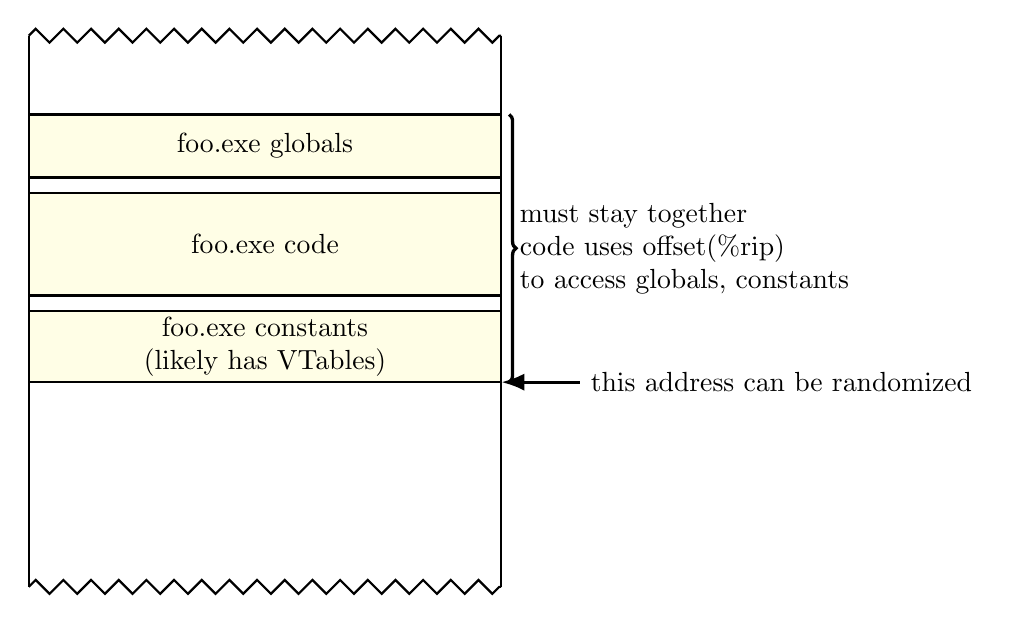
\begin{tikzpicture}[remember picture]
\draw[thick,decorate,decoration={zigzag}] (0, 0) -- (6, 0);
\draw[thick] (0, 0) -- (0, -7);
\draw[thick] (6, 0) -- (6, -7);
\draw[thick,decorate,decoration={zigzag}] (0, -7) -- (6, -7);
\draw[thick,fill=yellow!10] (0, -1) rectangle ++(6, -0.8) node[midway] {foo.exe globals};
\draw[thick,fill=yellow!10] (0, -2) rectangle ++(6, -1.3) node[midway] {foo.exe code};
\draw[thick,fill=yellow!10] (0, -3.5) rectangle ++(6, -0.9) node[midway,align=center] {foo.exe constants \\ (likely has VTables)};
\draw[very thick,Latex-] (6, -4.4) -- ++ (1cm, 0cm) node[right] {this address can be randomized};
\draw[very thick,decorate,decoration={brace,mirror}] (6.1, -4.4) -- ++ (0cm, 3.4) node[midway,right,align=left] {
    must stay together \\
    code uses offset(\%rip) \\
    to access globals, constants
};
\end{tikzpicture}
\end{frame}

